\section{Data}

We used the Media Forensics Challenge 2018 Dataset \cite{guan2019mfc} to perform our experiments. Each entry in the dataset 
is uniquely identified using a 32 character unique string. Each entry has 3 parts in it, a probe image, target image and a 
indicator images. The probe image, shown in Figure \ref{fig:probe_image}, is the original image with the manipulation in it. 
The target image, shown in Figure \ref{fig:target_image}, is a black and white
image, in which the black pixels represent manipulated areas and white pixels represent non-manipulated.
As mentioned before, the algorithms that perform image manipulation localization are called indicators and the output image 
from these algorithms are 
called indicator images. The indicator images, a few shown in Figure \ref{fig:indicator_images}, are the output images
produce from the indicators that ran on this probe 
image. To reduce the computational costs of our experiments, we downscaled the original dataset by a factor of 40. 

\begin{figure}
    \centering
    \begin{subfigure}{.49\textwidth}
    \centering
      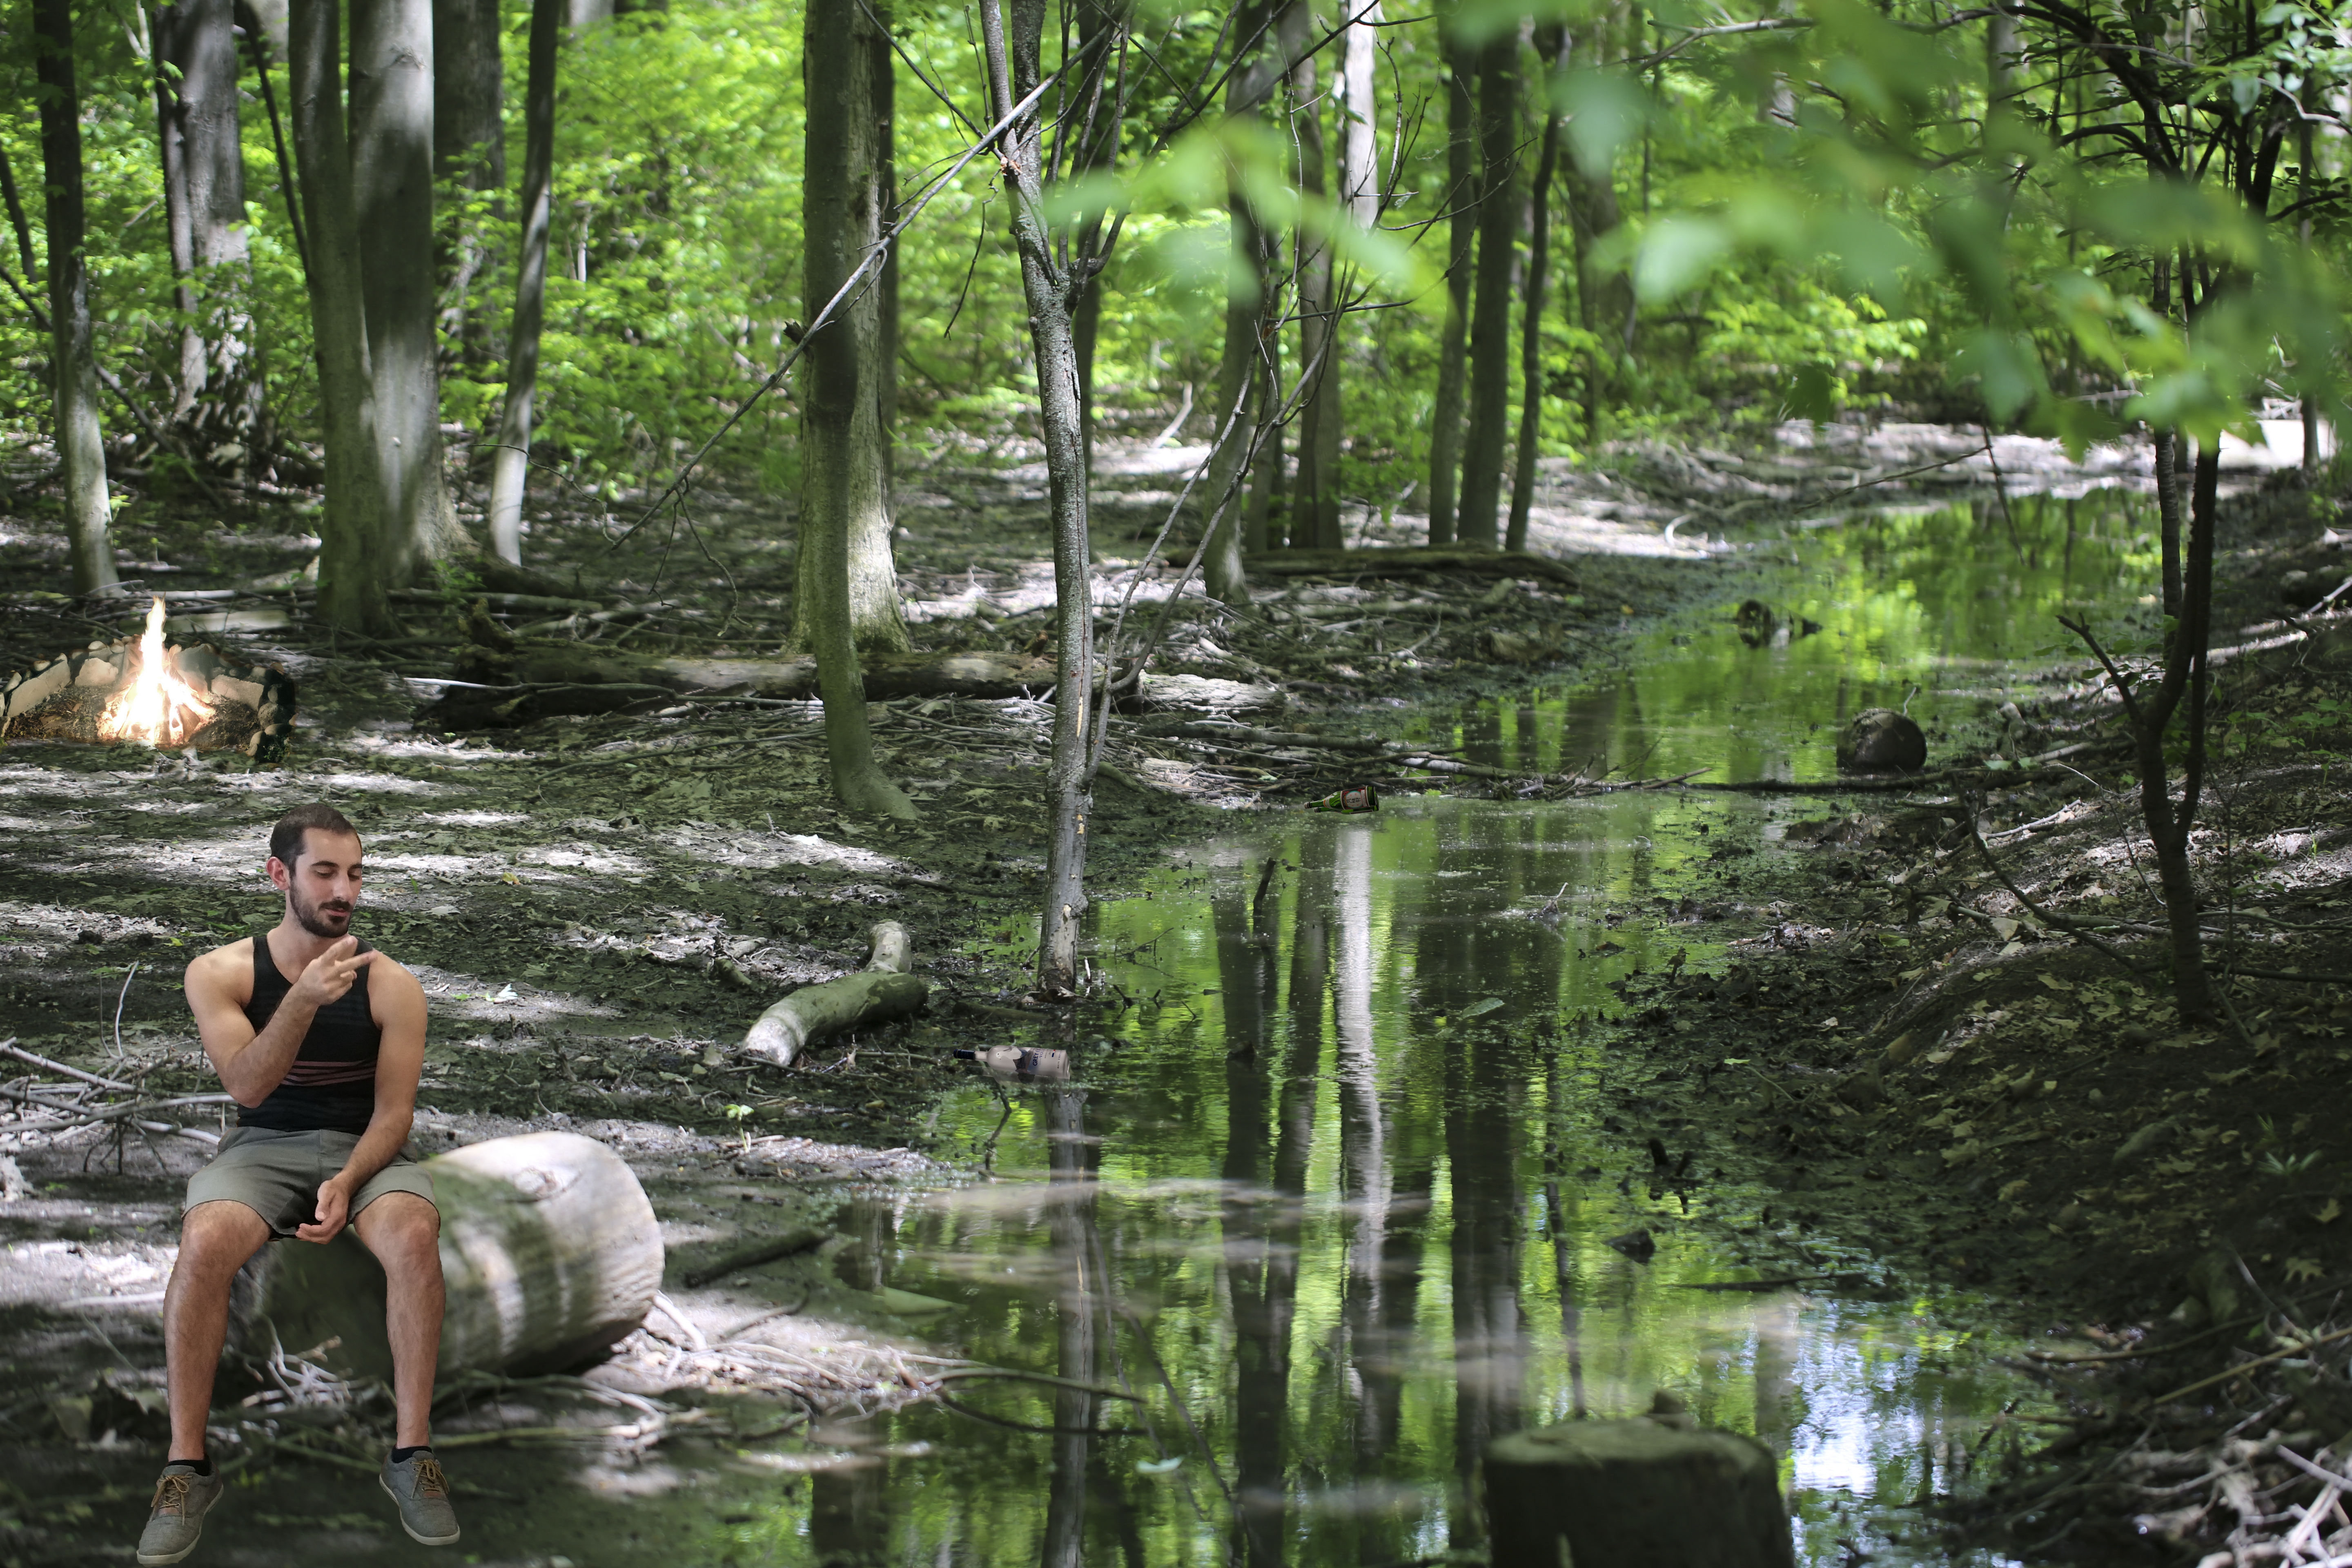
\includegraphics[width=.8\linewidth]{figures/probe_image.jpg}
      \caption{Probe Image}
      \label{fig:probe_image}
    \end{subfigure}
    \begin{subfigure}{.49\textwidth}
    \centering
      \frame{\includegraphics[width=.8\linewidth]{figures/target.png}}
      \caption{Target Image}
      \label{fig:target_image}
    \end{subfigure}
    \caption{Probe and Target image of a row of data}
    \label{fig:probe_target_image}
\end{figure}


\begin{figure}
    \centering
    \begin{subfigure}{.48\textwidth}
    \centering
      \includegraphics[width=.8\linewidth]{figures/ind1.png}
    \end{subfigure}
    \begin{subfigure}{.48\textwidth}
    \centering
      \includegraphics[width=.8\linewidth]{figures/ind2.png}
    \end{subfigure}
    \begin{subfigure}{.48\textwidth}
        \centering
      \includegraphics[width=.8\linewidth]{figures/ind3.png}
    \end{subfigure}
    \begin{subfigure}{.48\textwidth}
        \centering
      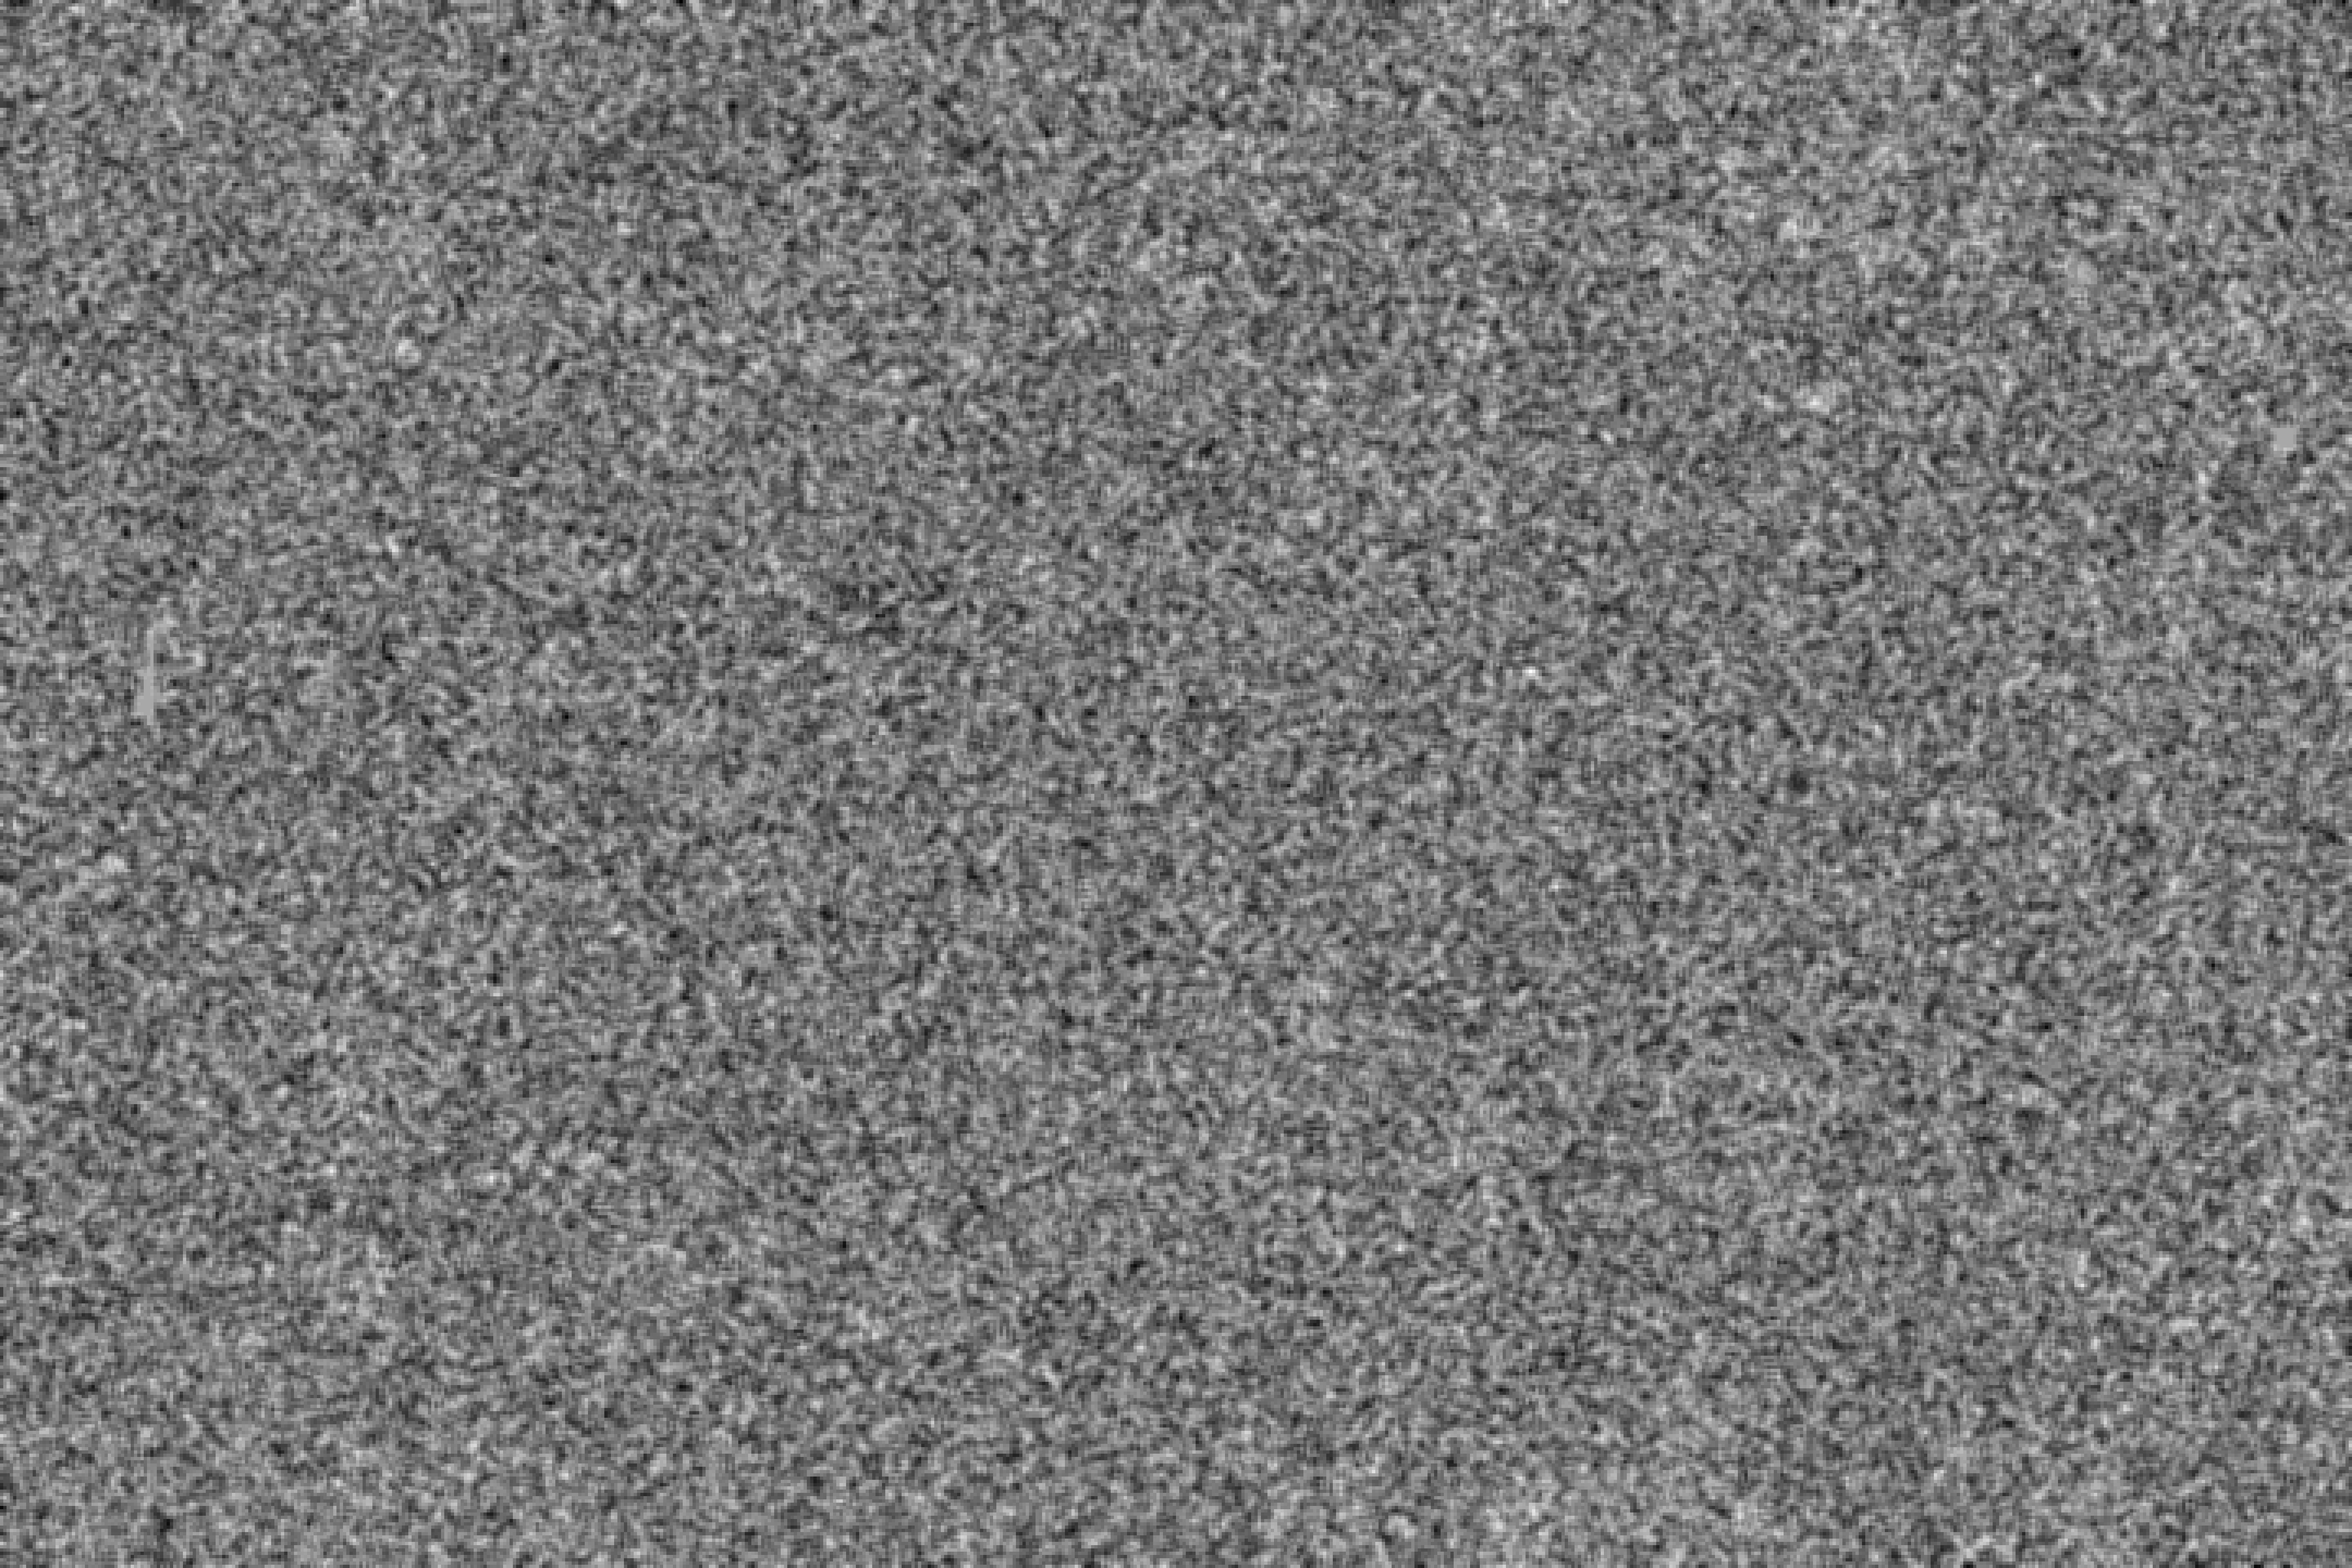
\includegraphics[width=.8\linewidth]{figures/ind4.png}
    \end{subfigure}
    \caption{A few indicator images}
    \label{fig:indicator_images}
\end{figure}

\subsection{Exploratory Data Analysis}

To better understand the data and its properties, some simple data exploration steps have been performed. Since the core 
task is localization of manipulations, it is very important to get an idea of the distribution of the percentage of 
manipulated pixels in the probe images. To visualize this, for each image we calculated the fraction of image pixels that 
were manipulated with respect to the whole image and plotted a pie chart of the distrubtion in Figure 
\ref{fig:manipulation_fractions}, which shows that most of the images have very little
manipulation in them. The skewness in the amount of manipulation is a major factor that we have to take in consideration 
when designing the models and interpreting the results.

\begin{figure}
    \centering
    \includegraphics[width=\textwidth]
        {figures/manipulation_fractions_0_-1.png}
    \caption{Manipulation Fractions}
    \label{fig:manipulation_fractions}
\end{figure}

The distribution of the size of images is another important factor to consider and to visualize this a graph of the 
frequency of the image dimensions have been plotted in Figure \ref{fig:dimension_distribution_graph}, which shows 
that there is skewness here as well.

\begin{figure}
    \centering
    \includegraphics[width=\textwidth]
        {figures/image_distribution_0_-1.png}
    \caption{Image Dimension Frequency Distribution}
    \label{fig:dimension_distribution_graph}
\end{figure}
